\subsection{Notations and Problem Formulation}

A trajectory $\xi$ is a sequence of poses in the Cartesian space  ... starting from $S$.



\subsection{Legibility Score}

The original formula for motion legibility (by Dragan et al. \cite{dragan2013legibility}) for an observed trajectory $\xi$ \cite{dragan2013legibility} is as follows:

\begin{equation}
    \label{eq_dragan9}
    \text { legibility }(\xi)=\frac{\int P\left(G^* \mid \xi_{S \rightarrow \xi(t)}\right) f(t) d t}{\int f(t) d t}
\end{equation}

\noindent
This equation assumes $P\left(G \mid \xi_{S \rightarrow \xi(t)}\right)$ is the way an observer distributes probabilities to potential goals of the robot, with $G^*$ being the true goal of the robot, and $f(t)$ to be a descending function like $f(t)=T-t$ which assigns higher weights to the initial parts of the trajectory, justifying the fact that a legible motion should minimize the ambiguity as soon as possible for the observers.

To compute Eq. (\ref{eq_dragan9}), they use the Bayse' rule and rewrite $P\left(G^* \mid \xi_{S \rightarrow \xi(t)}\right)$ as below:

\begin{equation}
    \label{eq_dragan8} 
    P\left(G \mid \xi_{S \rightarrow Q}\right) \propto \frac{\exp \left(-C\left(\xi_{S \rightarrow Q}\right)-C\left(\xi_{Q \rightarrow G}^*\right)\right)}{\exp \left(-C\left(\xi_{S \rightarrow G}^*\right)\right)} P(G)
\end{equation}

with $P(G)$ being a prior distribution of the potential goals and $C(\xi)$ being a cost function for an observed trajectory $\xi$ or an optimal trajectory $\xi^*$. In the original work of Dragan et al. \cite{dragan2013legibility} however, this is considered as a Euclidean distance between the initial and the goal point for the latter, which makes it too simplistic, i.e. a real human might use his own knowledge and reasoning for predicting the robot's goal based what they observe and making this simple assumption is not always aligned with human actualities.


% \begin{figure}
%     \centering
%     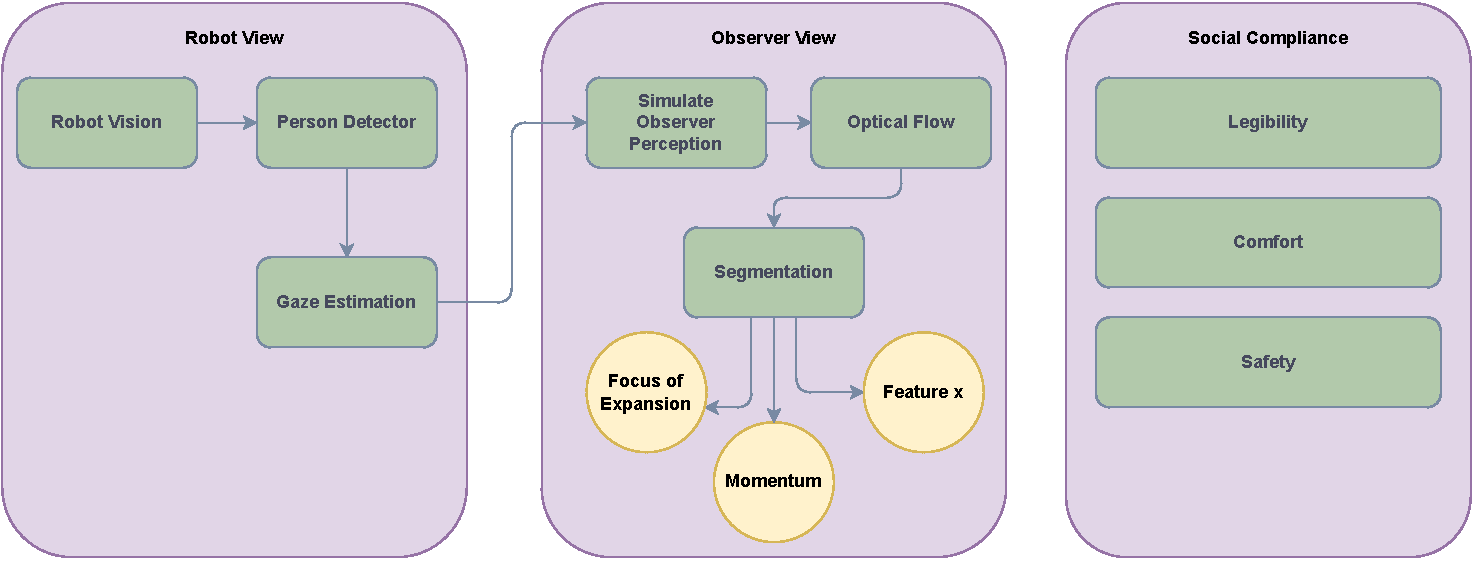
\includegraphics[width=0.8\textwidth]{figs/Legibot-fig1.pdf}
%     \caption{Overview}
%     \label{fig:enter-label}
% \end{figure}

\subsection{Short-term Motion Prediction using Optical Flow}
Optical flow is a technique used to analyze the apparent motion of objects in an image or a sequence of images. It estimates the motion of objects by tracking how pixels move from one frame to another.


\begin{equation}
I_x(u, v) \cdot V_x + I_y(u, v) \cdot V_y + I_t(u, v) = 0 
\end{equation}

\noindent 
where
$I_x(u, v)$, $I_y(u, v)$ and $I_t(u, v)$ are respectively, image gradient in the x-direction, y-direction, and temporal derivative and $V_x$ and $V_y$ are horizontal and vertical components of the optical flow vector, respectively.

% \begin{figure}
%     \centering
%     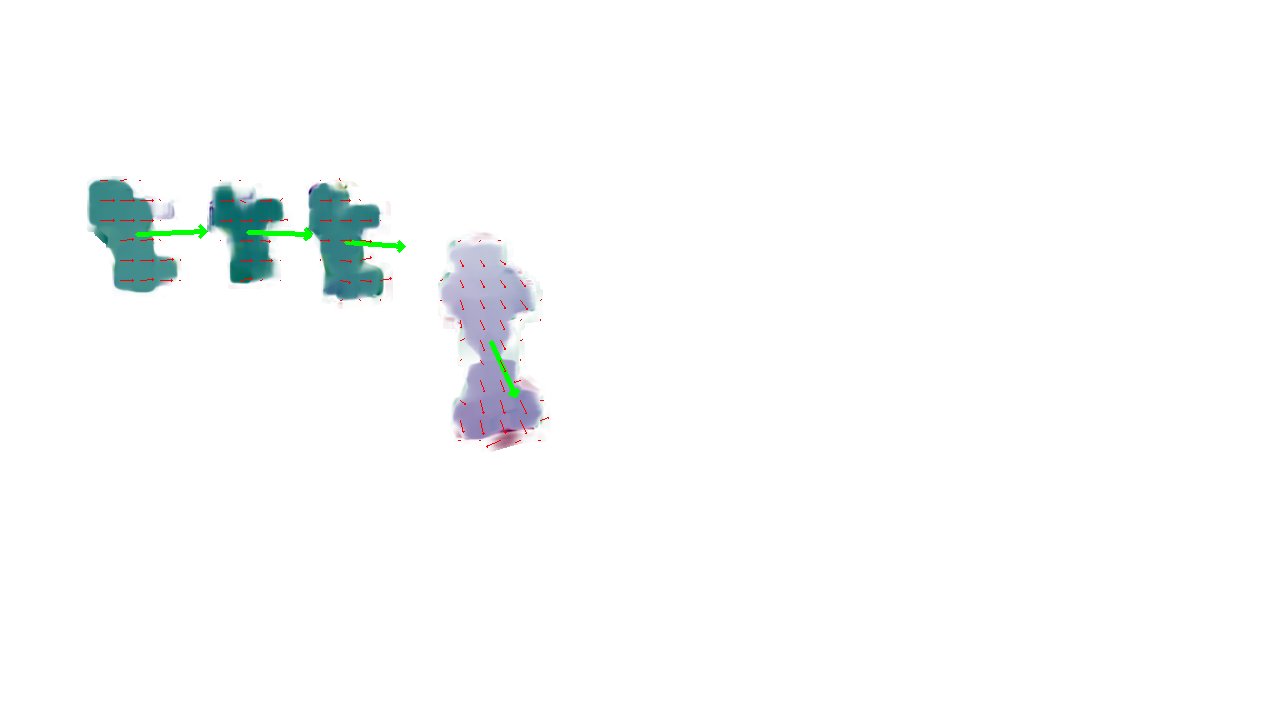
\includegraphics[width=0.6\textwidth]{figs/Pepper-optical-flow.png}
%     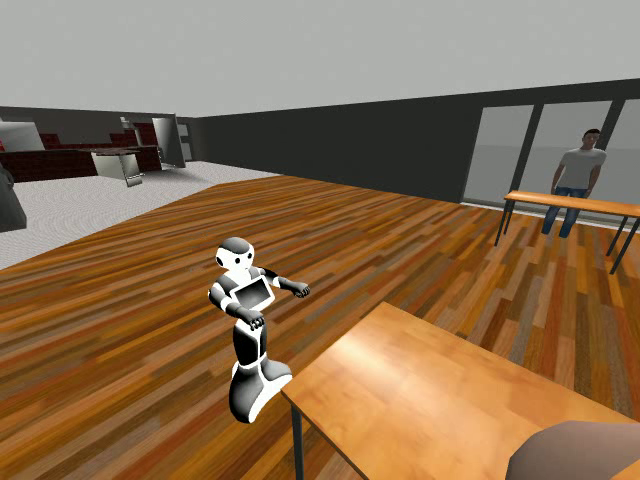
\includegraphics[width=0.4\textwidth]{figs/legibot-pepper-restaurant.png}
%     \caption{Sample Optical Flow}
%     \label{fig:enter-label}
% \end{figure}

\begin{figure}[ht]
  \centering
  \begin{subfigure}{0.5\textwidth}
    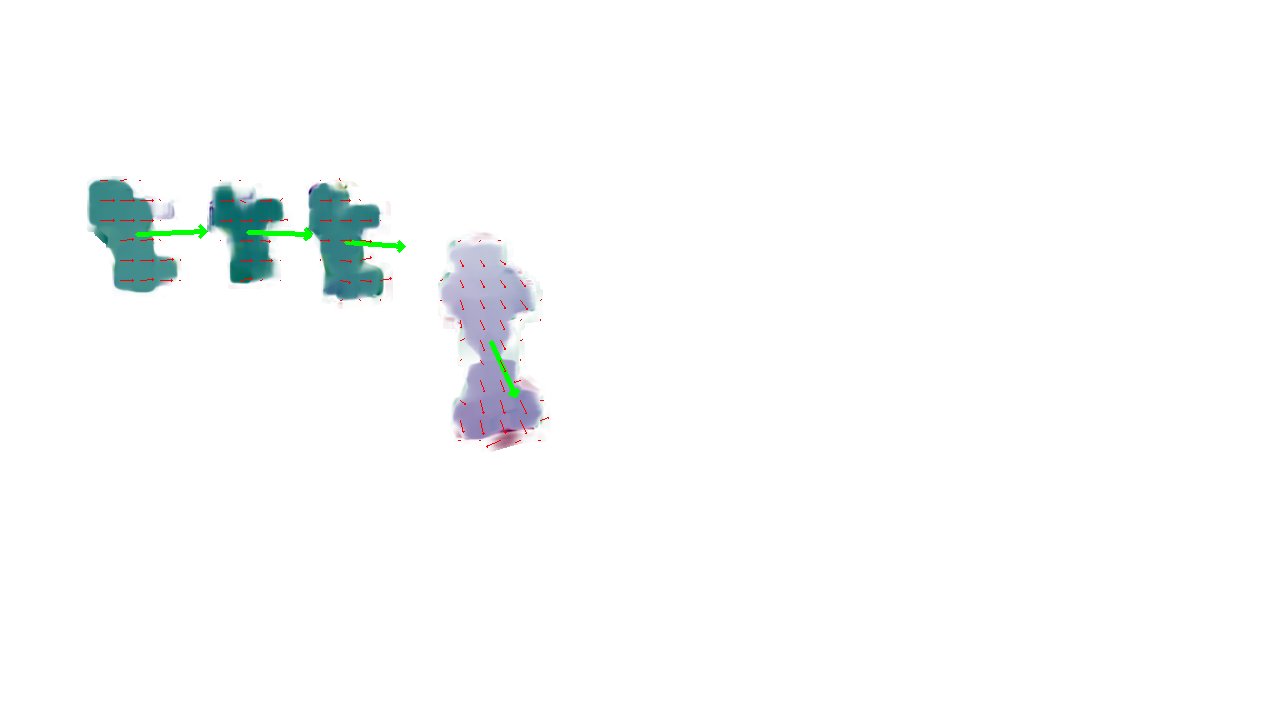
\includegraphics[width=\linewidth]{figs/Pepper-optical-flow.png}
    \caption{Sequence of Optical Flow outputs for the robot motion}
    \label{fig:sub1}
  \end{subfigure}
  \hspace{0.05\textwidth}
  \begin{subfigure}{0.35\textwidth}
    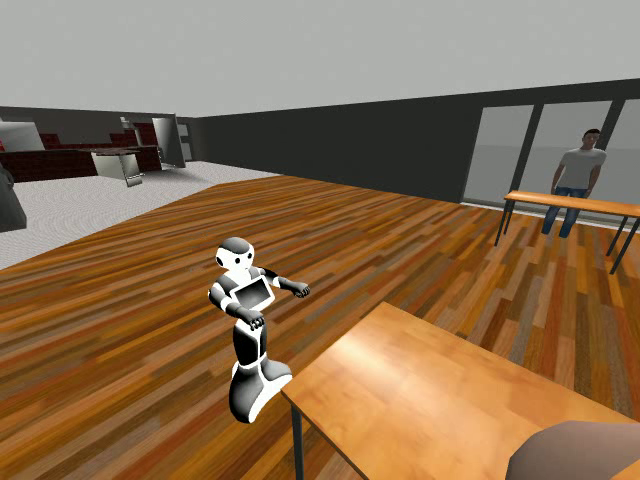
\includegraphics[width=\linewidth]{figs/legibot-pepper-restaurant.png}
    \caption{Normal View}
    \label{fig:sub2}
  \end{subfigure}
  \caption{Observer View}
  \label{fig:main}
\end{figure}

% Post-process
The process of calculating the optical flow image from the observer's perspective begins with capturing the frames as the observer. Optical flow algorithms analyze the pixel-level displacements between consecutive frames to estimate the apparent motion of objects within the scene. In the post-processing phase, we analyze the optical flow image to segment objects and distinguish the robot's motion. This segmentation and motion distinction process is essential ...

% \hl{See this:} \cite{park2023VRSickness} and \cite{gil2016estimating}

% \subsection{Focus of Expansion}

% The Focus of Expansion (FoE) $F_i$ in optical flow imagery refers to a specific point or region within the image where all optical flow vectors appear to converge. It is a concept used in computer vision and motion analysis to understand the motion of objects in a scene. 
% Theoretically, all we need are two vectors since we can simply take the lines defined by these two vectors and determine where they meet. This will be the focus of expansion. Of course, in reality, noise and other errors from the many steps to reach this point will result in imperfect optical flow vectors. Instead, the following formula considers a set of $n$ flow vectors \hl{$\{(v_i, u_i)\}$} from the detected object:

% \begin{equation}
% \begin{aligned}
% \mathfrak{F} & =\left(A^{T} A\right)^{-1} A^{T} \mathbf{b}
% \end{aligned}
% \end{equation}

% \noindent
% where
%     \begin{equation}
%     A=\left[\begin{array}{cc}
%     v_{0} & u_{0} \\
%     \cdots & \cdots \\
%     v_{n} & u_{n}
%     \end{array}\right] ,
%     \quad \mathbf{b}=\left[
%     \begin{array}{c}
%     b_{0} \\
%     \cdots \\
%     b_{n}
%     \end{array}\right]    
% \end{equation}

% \noindent
% and for each pixel $p_{i}=(x, y)$, 
% %the associated flow vector $\mathbf{v}=(u, v)$ gives $v_{i}=v, u_{i}=u$,  
% $b_{i}=x v-y u$.
% %
% \noindent
% It can finally be rewritten as:
% \begin{equation}
% \begin{aligned}
% \mathfrak{F} & =\
% \left[\begin{array}{c}
% \sum v_{i} b_{i} \sum u_{j}^{2}-\sum u_{i} b_{i} \sum v_{j} u_{j} \\
% -\sum v_{i} b_{i} \sum u_{j} v_{j}+\sum u_{i} b_{i} \sum u_{j}^{2}
% \end{array}\right]
% & -\frac{1}{\sum u_{j}^{2} v_{j}^{2}-\left(\sum v_{i} u_{i}\right)^{2}}
% \end{aligned}
% \end{equation}

% \noindent
% \textbf{TODO:} Move these equations to an appendix

% \begin{figure}
%     \centering
%     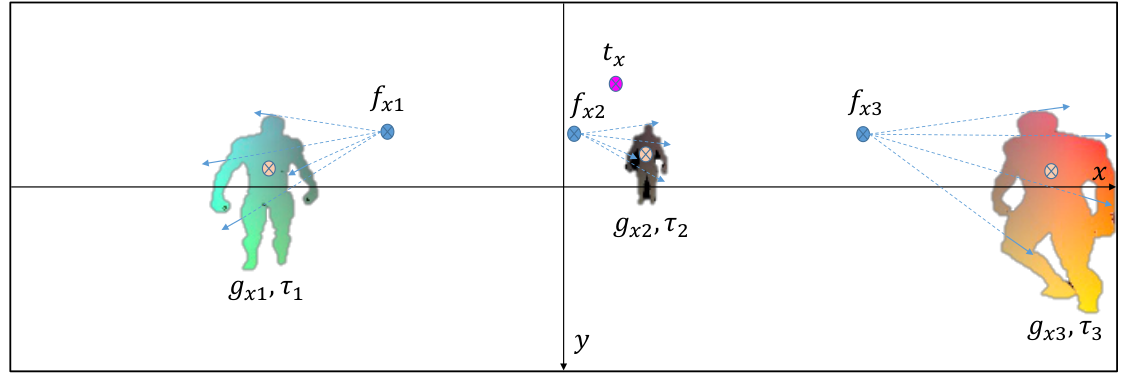
\includegraphics[width=0.5\textwidth]{figs/sample-FoE.png}
%     \caption{Focus of Expansion Example}
%     \label{fig:enter-label}
% \end{figure}

\subsection{Direction of Motion}
% The FoE does not always show where the robot is heading, for example when an object is approaching the observer, the motion lines would converge behind the moving object, and the FoE can be misleading. \\
% Then ...

% \hl{the image of this vector on the image plane is called the Focus of Expansion (FoE) when the camera moves forwards, or the Focus of Contraction (FoC) when it moves backward, see Fig. 1. Although FoE and FoC refer to opposite directions, their properties are very similar}

% \sethlcolor{cyan}
% \hl{
    Compute the DoM of the robot and calculate the difference between the direction of FoE vector and the robot-to-goal[i] direction.  This can be a metric to assess the legibility of the robot's motion w.r.t the potential goals in the environment.
% }
% \sethlcolor{yellow}




